\documentclass[aspectratio=169]{beamer}
\usetheme{hogent}
\usecolortheme{hgwhite} % witte achtergrond, zwarte tekst

%% common.tex -- Code die in elk .tex-bestand terug komt

%% Packages

\usepackage[dutch]{babel}
\usepackage{graphicx}
\usepackage{comment,enumerate,hyperref}
\usepackage{amsmath,amsfonts,amssymb}
\usepackage{eurosym}
\usepackage{booktabs}
\usepackage{multicol,multirow}
\usepackage{listings}

\usepackage[outputdir=out]{minted}
%\usepackage{minted}

\usepackage[backend=biber,style=apa]{biblatex}
\DeclareLanguageMapping{dutch}{dutch-apa}

\usepackage{csquotes}

%% Variabelen, elk academiejaar aan te passen
\newcommand{\academicyear}{2023--2024 (revisie: \today)}
\newcommand{\lecturers}{Thomas Aelbrecht \and Thomas Parmentier \and Bert Van Vreckem}
\newcommand{\coursename}{Research Methods (IT)}

%% Macro's en commando's

%% \alertbox: een kader voor tekst die moet opvallen
\newcommand{\alertbox}[2][hgblue]{%
  \setbeamercolor{alertbox}{bg=#1,fg=white}
  \begin{beamercolorbox}[sep=2pt,center]{alertbox}
    \textbf{#2}
  \end{beamercolorbox}
}

\usepackage{wasysym}

%---------- Info over de presentatie ------------------------------------------

\title{Module 5. Research methods.}
\subtitle{\coursename}
\author{\lecturers}   % Pas waarden aan in common.tex
\date{\academicyear}

\begin{document}

\begin{frame}
  \maketitle
\end{frame}

\begin{frame}
  \frametitle{Content}

  \tableofcontents
\end{frame}

\begin{frame}
  \frametitle{Objective}

  \begin{itemize}
    \item Writing out a methodology/action plan
    \item How to tackle typical thesis subjects
    \item Proof-of-concept (POC)
    \item Collecting quantitative data
    \item Pitfall: the questionnaire
  \end{itemize}
\end{frame}

\section{Action plan}

\begin{frame}
  \frametitle{Methodology}

  \begin{itemize}
    \item = part of your bachelor thesis proposal
    \item writing an action plan
          \begin{itemize}
            \item Split into phases
            \item Research techniques used
            \item Objective/result of each phase
            \item Order/Dependencies
            \item Timing
          \end{itemize}
  \end{itemize}

  \alertbox{The more detailed your action plan, the easier it is to get started!}

\end{frame}

\begin{frame}
  \frametitle{Example}
  \small
  To start off the research, an investigation will be conducted how to create a design system, by building a simple component library from an existing library and using it to set up a design system. This will also help to gain a better understanding of the other research questions. Second, a comparative study will be performed on component libraries and design systems, and where and when you use them with some examples. Finally, the advantages of an own design system will be investigated by conducting some interviews with employees of companies that have implemented it. A questionnaire will therefore be written, also pointing out the disadvantages of a design system, and proving a design system worthwhile or not.

\end{frame}

\begin{frame}
  \frametitle{Common mistakes}

  \begin{itemize}
    \item Insufficiently elaborated
    \item Sequence of phases is incorrect (e.g.\ start with proof-of-concept)
    \item Too vague (e.g.\ ``research'')
    \item Unsuitable techniques
    \item Unmeasurable or subjective criteria (e.g.\ `user-friendliness', `popularity')
    \item A priori choices
    \item Generated by LLM
    \item \ldots
  \end{itemize}

\end{frame}


\begin{frame}
  \frametitle{How to write an action plan?}

  \begin{itemize}
    \item Divide your research into phases
    \item Explain in depth per phase
          \begin{itemize}
            \item What you will do
            \item The result of this phase (artefact)
          \end{itemize}
    \item Visualize the action plan (e.g.\ flowchart or Gantt chart)
  \end{itemize}
\end{frame}

\section{Performing a comparative study}

\begin{frame}
  \frametitle{Phases}

  \alertbox{Always start with a specific case!}

  \begin{itemize}
    \item Collecting requirements
    \item Long list
    \item Short list
    \item Proof-of-Concept
    \item Conclusions
  \end{itemize}

\end{frame}

\begin{frame}
  \frametitle{Collecting requirements}

  \begin{itemize}
    \item \textbf{Objective:} List minimal criteria for a good solution
    \item \textbf{Techniques:}
          \begin{itemize}
            \item Interviews with stakeholders (e.g.\ co-promoter?)
            \item MoSCoW method (must have, should have, etc.)
          \end{itemize}
    \item \textbf{Result:} list of requirements
          \begin{itemize}
            \item Ordered by importance
            \item Functional/non-functional
          \end{itemize}
  \end{itemize}

\end{frame}

\begin{frame}
  \frametitle{Long list}

  \begin{itemize}
    \item \textbf{Objective:} List options
    \item \textbf{Technique:} literature search
          \begin{itemize}
            \item Collect as many options as possible, don't exclude anything beforehand!
            \item Check against requirements, based on available information
          \end{itemize}
    \item \textbf{Result:} list with all options found (with reference)
  \end{itemize}

\end{frame}

\begin{frame}
  \frametitle{Short list}

  \begin{itemize}
    \item \textbf{Objective:} Selection of most interesting options
    \item \textbf{Technique:} Requirements/options summary table
    \item \textbf{Result:} Choice of 1 or some options to elaborate further
  \end{itemize}

\end{frame}

\begin{frame}
  \frametitle{Example}
  \framesubtitle{Requirements summary table}

  \centering
  \begin{tabular}{cccc|cc|cccc}
    \toprule
    Option & \multicolumn{3}{c}{M} & \multicolumn{2}{c}{S} & \multicolumn{4}{c}{C}                                                             \\ \midrule
    A      & \CIRCLE               & \CIRCLE               & ?                     & \CIRCLE & ?       & \CIRCLE & \CIRCLE & ?       & \CIRCLE \\
    B      & \CIRCLE               & ---                   & \CIRCLE               & ---     & \CIRCLE & \CIRCLE & \CIRCLE & \CIRCLE & \CIRCLE \\
    C      & \CIRCLE               & \CIRCLE               & \CIRCLE               & \CIRCLE & ---     & \CIRCLE & \CIRCLE & \CIRCLE & ---     \\ \bottomrule
  \end{tabular}

  \bigskip

  (\CIRCLE = requirement met; --- = requirement not met; ? = no info available)

\end{frame}

\begin{frame}
  \frametitle{Proof-of-concept}

  \begin{itemize}
    \item \textbf{Objective:} Validate whether the best option can solve the problem.
    \item \textbf{Technique:} Test setup/proof-of-concept
    \item \textbf{Result:} Prototype of ICT solution for the problem from the research question
  \end{itemize}

\end{frame}

\begin{frame}
  \frametitle{Drawing conclusions}

  \begin{itemize}
    \item Recommend the best possible option
    \item Identify remaining gaps
  \end{itemize}
\end{frame}

\section{Cybersecurity: risk assessment}

\begin{frame}
  \frametitle{Cybersecurity related topics}

  From students' proposals:

  \begin{itemize}
    \item Which cyber attacks are most frequent?
    \item How does password cracking work?
    \item How can companies/persons protect themselves?
    \item I want to do ``something'' on cybersecurity
  \end{itemize}

  \bigskip

  \alertbox{A bachelor thesis on cybersecurity is best when it handles a specific case!}

\end{frame}

\begin{frame}
  \frametitle{Problems with cybersecurity approach}

  \begin{itemize}
    \item Not systematic
          \begin{itemize}
            \item $\Rightarrow$ focus on less important aspects
          \end{itemize}
    \item Not thorough
          \begin{itemize}
            \item Firewall on the router is insufficient!
          \end{itemize}
    \item Budget
          \begin{itemize}
            \item Costs without ROI
          \end{itemize}
    \item Unproductive measures
          \begin{itemize}
            \item eg\ password policy
          \end{itemize}
  \end{itemize}

\end{frame}

\begin{frame}
  \frametitle{A cybersecurity case}

  \begin{itemize}
    \item One specific company
    \item A specific type of server/device
          \begin{itemize}
            \item e.g.\ ActiveDirectory, web application server, \ldots
            \item e.g.\ (edge) router, firewall, \ldots
          \end{itemize}
    \item A specific (web) application
          \begin{itemize}
            \item e.g.\ webapps from IT courses?
          \end{itemize}
  \end{itemize}

\end{frame}

\begin{frame}
  \frametitle{Systematic approach: risk assessment}

  Jackson, C. (2010) \textit{Network Security Auditing.} Cisco Press.

  \begin{enumerate}
    \item Describe system
    \item List current measures
    \item Identify threats
    \item Identify weaknesses
    \item Estimate probability
    \item Estimate Impact
    \item Determine risk
    \item Formulate recommendations
  \end{enumerate}

\end{frame}

\begin{frame}
  \frametitle{System description}

  \begin{itemize}
    \item How? Stakeholder Interview
    \item List hardware, software, equipment, services, \ldots
    \item Set up schedule/overview
    \item What data?
  \end{itemize}

\end{frame}

\begin{frame}
  \frametitle{Threat identification}

  \begin{itemize}
    \item How?
          \begin{itemize}
            \item Interview with stakeholders
            \item Literature study
          \end{itemize}
    \item Describe possible attack scenarios
  \end{itemize}

\end{frame}

\begin{frame}
  \frametitle{Weakness identification}

  \begin{itemize}
    \item How? Experiment
          \begin{itemize}
            \item Set up test environment!
            \item Avoid production systems.
          \end{itemize}
    \item Pen-testing techniques
    \item Vulnerability scanning
          \begin{itemize}
            \item eg OWASP ZAP, Wapiti, OpenVAS, Lynis, \ldots
          \end{itemize}
    \item Fuzzing
    \item \ldots
  \end{itemize}

\end{frame}

\begin{frame}
  \frametitle{List current measures}
  \begin{itemize}
    \item Interview with stakeholders
    \item Access protection, levels
    \item Security policy (e.g.\ passwords, etc.)
  \end{itemize}

\end{frame}

\begin{frame}
  \frametitle{Risk assessment}

  \centering

  Risk = Probability $\times$ impact

  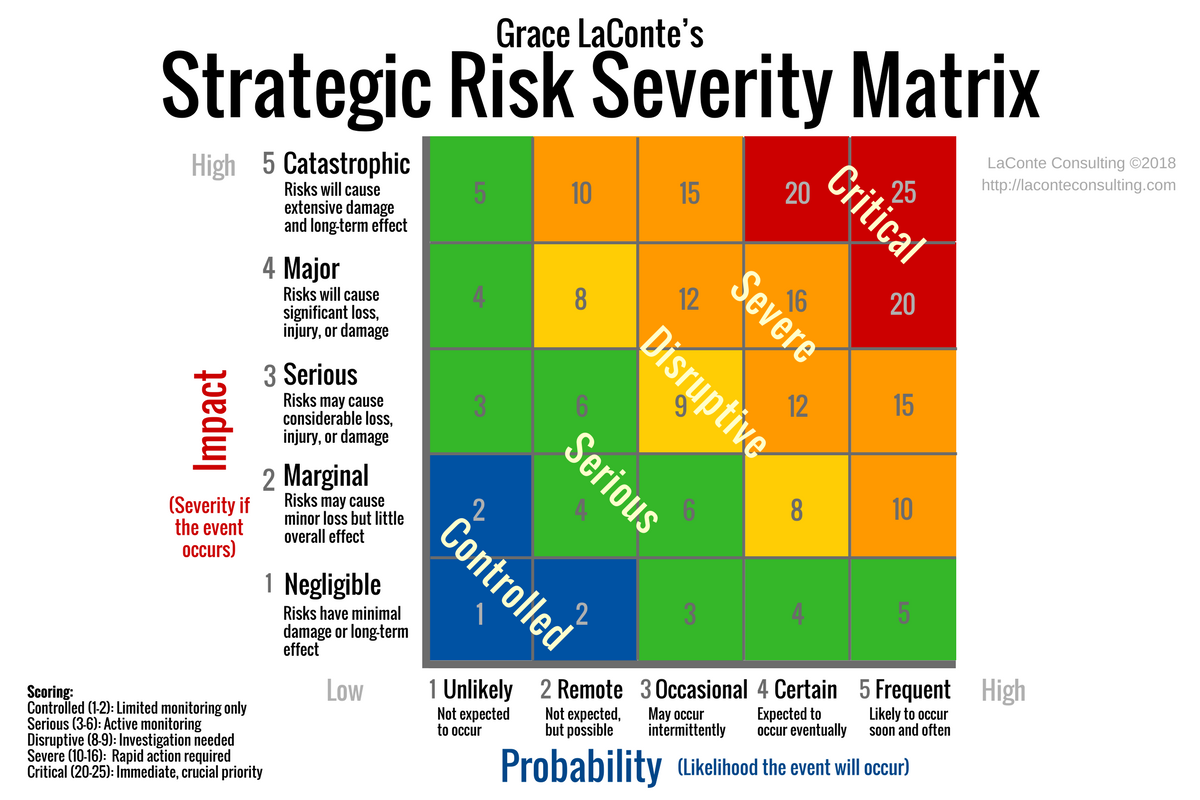
\includegraphics[height=.7\textheight]{5/risk-severity-matrix}

\end{frame}

\begin{frame}
  \frametitle{Recommendations}

  \begin{columns}
    \begin{column}{.5\textwidth}
      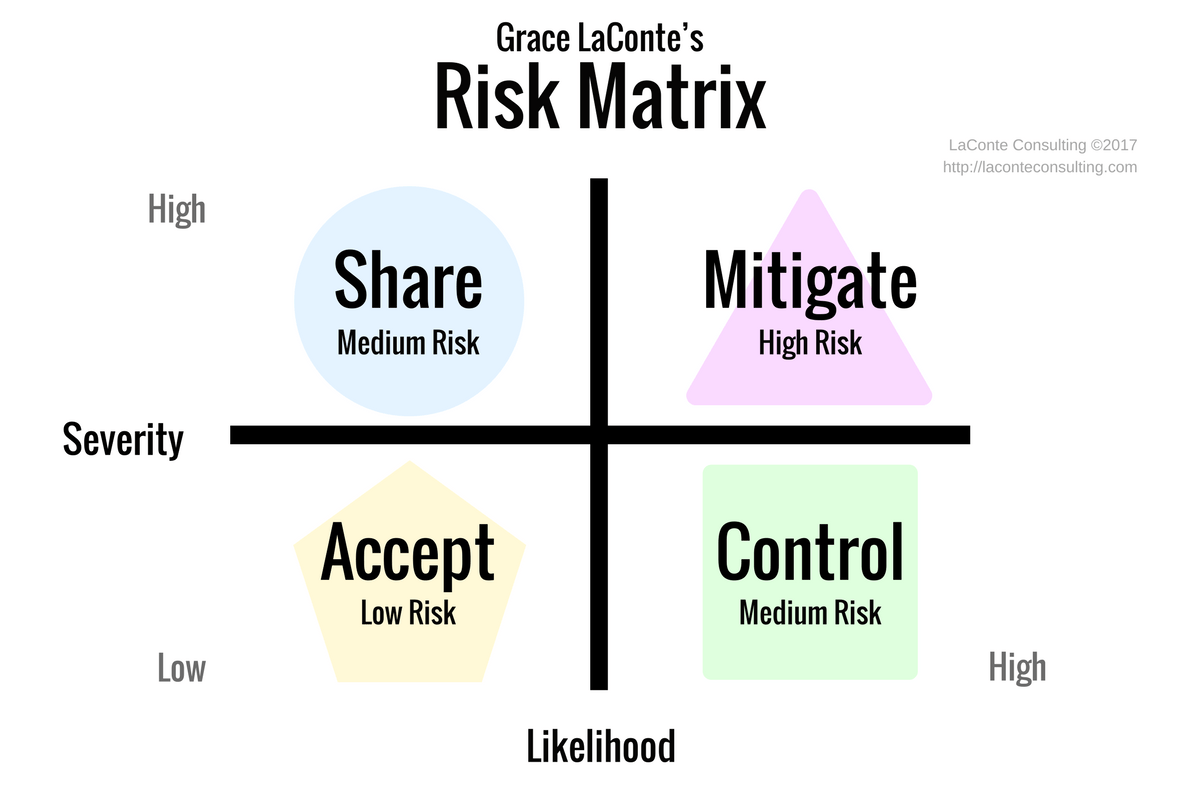
\includegraphics[width=\textwidth]{5/risk-matrix-severity-and-likelihood.png}
    \end{column}

    \begin{column}{.5\textwidth}
      \begin{itemize}
        \item \textbf{Mitigate:} Take action, solve problem
        \item \textbf{Control:} Transfer to another entity (e.g.\ outsource to IT service provider, security specialists)
        \item \textbf{Share:} Take insurance
        \item \textbf{Accept:} Do nothing
      \end{itemize}
    \end{column}
  \end{columns}
\end{frame}

\section{Data Engineering subject}

\begin{frame}
  \frametitle{BP Data Engineering}

  Typically: applying AI/ML techniques in a concrete case/situation

  E.g.

  \begin{itemize}
    \item Automatic scoring of a darts board
    \item Anomaly detection in server monitoring
    \item Summarizing study materials for students with learning disabilities
    \item \ldots
  \end{itemize}

\end{frame}

\begin{frame}
  \frametitle{Types of sources}

  \begin{description}
    \item[Review papers] overview of research/techniques in a specific problem domain
    \item[Research papers] new research results, methodology, experiments
  \end{description}

\end{frame}

\begin{frame}[plain]
  \frametitle{Procedure}

  \begin{itemize}
    \item Define the concrete \textit{learning task}
    \begin{itemize}
      \item What does your system need to learn?
      \item What input does it need and in what form?
      \item What does the output look like?
      \item Category? (Un)supervised/reinforcement learning?
    \end{itemize}
    \item Select (at least) one \textit{research paper} in advance
    \item Reproduce/adapt to your case using the methodology described in the paper
    \item Not working? Try another research paper in a next iteration!
  \end{itemize}

  \alertbox{Describe which research papers you will start with in your proposal!}
\end{frame}

\section{Proof-of-concept or test-setup}

\begin{frame}
  \frametitle{Proof-of-concept/test-setup}

  \begin{itemize}
    \item Objective:
          \begin{itemize}
            \item Demonstrate that the proposed solution is feasible
            \item Setup for conducting experiments
          \end{itemize}
    \item Important properties:
          \begin{itemize}
            \item Reproducibility
            \item Replicability
            \item Reusability
          \end{itemize}
  \end{itemize}

\end{frame}

\begin{frame}
  \frametitle{Reproducibility}

  \alertbox{Give the reader enough information to reproduce your test setup}

  \bigskip

  \begin{itemize}
    \item Which hardware? specs?
          \begin{itemize}
            \item Computers, network equipment, \ldots
          \end{itemize}
    \item Which software?
    \item Installation and configuration?
    \item Add image with test setup schedule!
  \end{itemize}

\end{frame}

\begin{frame}
  \frametitle{Replicability}

  \alertbox{You should be able to quickly build your set-up again}

  \bigskip

  \begin{itemize}
    \item Detailed procedure manual
    \item Automate! E.g.\ Vagrant, Docker
    \item Install script, config files, etc.\ in Github repo!
  \end{itemize}

\end{frame}

\begin{frame}
  \frametitle{Reusability}

  \alertbox{You can create similar variants of a test setup}

  \bigskip

  \begin{itemize}
    \item Compare options
    \item Compare configuration differences
  \end{itemize}

\end{frame}

\section{Quantitative data}

\begin{frame}
  \frametitle{Quantitative data collection}

  E.g.\ performance measurements

  \begin{itemize}
    \item Reproducible, replicable, reusable
    \item Automate experiments (e.g.\ shell script)
    \item Save results in convenient format
          \begin{itemize}
            \item Text based
            \item Computer readable
            \item e.g. CSV, JSON, YAML
          \end{itemize}
  \end{itemize}

\end{frame}

\begin{frame}
  \frametitle{Quantitative data processing}

  \begin{itemize}
    \item Use statistical software (Pyhon, R)
    \item Suitable visualization and analysis techniques
          \begin{itemize}
            \item See Data Science \& AI!
            \item Show variance in the data
            \item Apply statistical tests
          \end{itemize}
  \end{itemize}

\end{frame}

\begin{frame}
  \frametitle{Bivariate analysis: overview}
  \centering
  \begin{tabular}{lll}
    \toprule
    \textbf{Independent} & \textbf{Dependent} & \textbf{Test/Metric}    \\
    \midrule
    Qualitative          & Qualitative        & $\chi^2$-test           \\
                         &                    & Cramér's $V$            \\
    Qualitative          & Quantitative       & two-sample $t$-test     \\
                         &                    & Cohen's $d$             \\
    Quantitative         & Quantitative       & Regression, correlation \\
    \bottomrule
  \end{tabular}

  \bigskip

  \alertbox{There are more statistical techniques than the ones we've seen in DSAI!}
\end{frame}

\begin{frame}
  \frametitle{Quantitative data processing}

  Suppose the research question is ``Which DB system has the best performance: A or B?''

  \begin{itemize}
    \item<+-> Which experiment are you going to set up?
      % Test setup with DB A and B
      % Repeat queries on A and B, measure time
    \item<+-> What are the independent and dependent variables?
      % Independent: DB System (A or B)
      % Dep: response time
    \item<+-> What kind of graph would you use to visualize this?
      % boxplot, density diagram (kdeplot)
      % Bar chart of averages? ONLY IF YOU ALSO SHOW SPREAD using error bars, but this only makes sense if data is clearly normally distributed
    \item<+-> Which techniques can answer the research question?
      % t-test for 2 independent samples
  \end{itemize}


\end{frame}

\begin{frame}
  \frametitle{Tips when processing data}
  \begin{itemize}
    \item NEVER change raw data (CSV)
    \item Automate the workflow as much as possible
          \begin{itemize}
            \item Python script or Jupyter Notebook
            \item Import CSV
            \item Data cleaning
            \item Visualization
            \item Analysis
          \end{itemize}
    \item Keep track of your code in Git!
  \end{itemize}

  \alertbox{Think of reproducibility and replicability!}

\end{frame}

\section{Pitfall: the questionnaire}

\begin{frame}
  \frametitle{The questionnaire}

  \alertbox{For a bachelor thesis applied computer science a survey is usually not recommended!}

  \bigskip

  \begin{itemize}
    \item Often unsuitable for answering research question
    \item Often too few respondents
    \item Frequently unusable results
  \end{itemize}

\end{frame}

\begin{frame}
  \frametitle{Sampling}

  See also Data Science \& AI

  \begin{itemize}
    \item Well-defined population (sampling frame!)
    \item Random
    \item Sufficiently large
    \item Representative (stratified)
  \end{itemize}

\end{frame}

\begin{frame}
  \frametitle{Common problems}

  \begin{itemize}
    \item Population is not/poorly defined
    \item Sample is not random
          \begin{itemize}
            \item online survey
            \item convenience sampling
          \end{itemize}
    \item Very low response rate
    \item Bad questions $\Rightarrow$ useless answers
          \begin{itemize}
            \item Open questions
            \item Gauging opinion, not facts
          \end{itemize}
    \item No representativeness check
  \end{itemize}

\end{frame}

\section{Planning}

\begin{frame}
  \frametitle{Drawing up a schedule}

  \begin{itemize}
    \item Work with milestones and deadlines
    \begin{itemize}
      \item Duration e.g.\ `1w' is ambiguous
      \item Per week 4d internship, 1d thesis (no Easter holiday!)
      \item Take imposed deadlines into account
    \end{itemize}
    \item Milestone = delivery of an \textit{artefact}
    \begin{itemize}
      \item Finalizing a specific thesis chapter
      \item Implementation PoC/test setup/data workflow
      \item Executing tests, collecting results (CSV)
      \item \ldots
    \end{itemize}
  \end{itemize}

\end{frame}

\begin{frame}
  \frametitle{Imposed deadlines (23--24)}

  \begin{description}
    \item[2023--12--15] written proposal (feedback from supervisor by 2024--01--19)
    \item[2024--02--16] improved proposal
    \item[2024--03--22] draft literature review
    \item[2024--05--10] draft thesis
    \item[2024--05--24] final thesis
  \end{description}

  \medskip

  Adjust this yourself for AY 2024--2025!
\end{frame}

\begin{frame}[plain]
  \frametitle{Example: Gantt-diagram with deadlines}

  With Mermaid diagrams: \url{https://mermaid.js.org/syntax/gantt.html}

  \centering
  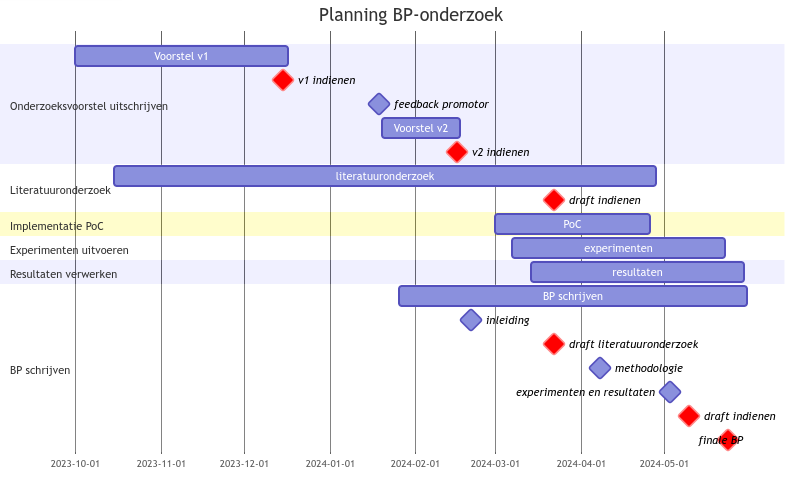
\includegraphics[height=.7\textheight]{5/gantt-deadlines.png}
\end{frame}

\begin{frame}
  \frametitle{Recommendations}

  \begin{itemize}
    \item Literature review phase can continue in parallel with following phases
    \item Apply \textit{agile} principles, work in iterations
    \item Schedule enough time for your own contribution!
    \item You should have built/implemented something before the Easter holidays
    \item Write the methodology yourself, don't let ChatGPT do it!
  \end{itemize}
\end{frame}
\section{Assignment}

\begin{frame}
  \frametitle{Writing the methodology}

  \begin{itemize}
    \item Write out action plan (Methodology)
    \item Divide research into different phases
          \begin{itemize}
            \item What exactly are you going to do?
            \item Why? What is the objective?
            \item What is the concrete result (artefact)?
            \item How are you going to do it (research method)?
          \end{itemize}
    \item Estimate milestones and deadlines
  \end{itemize}

\end{frame}

\end{document}
